\documentclass[11pt,a4paper]{article}
\usepackage[margin=1.1in]{geometry}
\usepackage{amsmath,amssymb}
\newcommand{\ZZ}{\mathbb{Z}}
\newcommand{\NN}{\mathbb{N}}
\usepackage[T1]{fontenc}
\usepackage{lmodern}
\usepackage{microtype}
\usepackage{booktabs}
\usepackage{parskip}
\usepackage{tikz}
\usetikzlibrary{arrows.meta,positioning,calc}
\usepackage{xcolor}
\definecolor{seclink}{HTML}{1F4E8C}
\definecolor{good}{HTML}{2A7A2A}
\definecolor{bad}{HTML}{B03030}
\definecolor{yellowbg}{HTML}{FBF3D5}
\usepackage[colorlinks=true,linkcolor=seclink,urlcolor=seclink]{hyperref}
\usepackage[most]{tcolorbox}
\tcbset{plainbg/.style={boxrule=0pt, sharp corners, colframe=white,
  left=4mm, right=4mm, top=3mm, bottom=3mm, before skip=3mm, after skip=3mm,
  parbox=false,
  before upper={\setlength{\parskip}{0.75\baselineskip}\setlength{\parindent}{0pt}}}}
\newtcolorbox{keybox}{plainbg, colback=yellowbg}

\title{\vspace{-2em}Three Programs in a Ring\\[0.4em]
\large the same experiment, in plain language}
\author{\normalsize Claude, for Robin}
\date{\normalsize 21 September 2026}

\begin{document}
\maketitle
\vspace{-1em}

\section*{1. Containers, and what a computation is}

\subsection*{Functions first}

A \textbf{function} $f$ from a set $A$ to a set $B$ is a rule which assigns, to
each element of $A$, exactly one element of $B$. Write $f : A \to B$.

Note what is fixed in advance: \emph{both} sets. Whichever $a$ you feed it, the
result is drawn from the same $B$. A function $\ZZ \to \ZZ$ returns an integer
whatever you give it.

\subsection*{Sets and types are the same thing here}

A \textbf{type} is the collection of values that something is permitted to be,
which is to say: a type is a set. The two words come from different traditions
and we will use whichever is less awkward --- ``set'' when the point is
mathematical, ``type'' when pointing at code --- but nothing changes when we
switch.

\[
  \mathrm{Bool} = \{0, 1\},
  \qquad
  \ZZ = \{\ldots, -2, -1, 0, 1, 2, \ldots\}
\]

A programmer who says a function \emph{returns a Bool} is saying the result is
an element of that two-element set. So $f : A \to B$ can be read as ``$f$ takes
an argument of type $A$ and returns a value of type $B$'', and the earlier
remark becomes: \emph{a function has one return type, fixed before you call
it}.

The responses in this experiment will form a two-element set as well,
$\{+1, -1\}$ --- the same type as $\mathrm{Bool}$, with different names for its
two elements.

\subsection*{A computer program is a function}

A program that takes an input and produces an output \emph{is} a function, from
the type of its inputs to the type of its outputs. A program which reads a
whole number and reports whether it is even is a function
$\ZZ \to \mathrm{Bool}$. Running the program is applying the function.

This stays true when the program is slow, and it stays true when the program
gets its answer by talking to another machine over a network. A program that
\emph{eventually} returns a $\mathrm{Bool}$ still returns a $\mathrm{Bool}$:
waiting is not a change of type. That is all a \texttt{Promise}
records, in the code below --- a value of a known type that has not arrived
yet.

So if each of our three programs accepted one prompt and returned one kind of
answer, there would be nothing more to say: each would be a function, and we
could stop here. The reason we cannot is the next paragraph.

\subsection*{Containers}

A \textbf{container} is given by:

\begin{itemize}
\item a set $P$, whose elements we call \textbf{prompts} (questions); and
\item for each prompt $p \in P$, a set $R(p)$, whose elements are the
      \textbf{responses} (answers) that are valid for \emph{that} prompt.
\end{itemize}

The second item is not a function into some set of responses. It assigns a
whole \emph{set} to each prompt, and different prompts may be assigned
different sets. That is the only subtlety in the definition, and it is the
whole point of it.

\begin{keybox}
\textbf{Example.} A library catalogue. $P$ contains the prompts \emph{how many
books are there?}, \emph{who wrote this one?} and \emph{is it on loan?}

\[
\begin{aligned}
R(\text{how many books are there?}) &= \NN \\
R(\text{who wrote this one?})       &= \text{names} \\
R(\text{is it on loan?})            &= \{\,\text{yes},\ \text{no}\,\}
\end{aligned}
\]

A response valid for one prompt is nonsense for another, and the container is
precisely the record of which goes with which.
\end{keybox}

\subsection*{What a computation is}

\begin{keybox}
A \textbf{computation} for a container is a rule which, given any prompt $p$,
produces one response belonging to $R(p)$.
\end{keybox}

Compare that with a function. If every prompt had the same response set $B$, a
computation would be exactly a function $P \to B$. It is not, because the set
the answer must come from \emph{moves as the prompt moves}. A computation is a
function whose output set depends on its input.

That is what it means to model computation with containers: the container is
the specification --- what may be asked, and what would count as an answer to
each thing that may be asked --- and a computation is anything that meets it.
Neither says how the answer is obtained.

\subsection*{Programs}

Now the part that does the work. Suppose you can prompt a container $D$, and
you want to provide a different container $C$ to somebody else.

A \textbf{program} from $C$ to $D$ is a pair:

\begin{enumerate}
\item a function $u : P_C \to P_D$ --- given a prompt of $C$, which prompt to
      send to $D$;
\item for each prompt $p$ of $C$, a function
      $f_p : R_D(u(p)) \to R_C(p)$ --- given $D$'s response to the prompt you
      sent, how to turn it into a valid response to the prompt you were
      actually asked.
\end{enumerate}

This is exactly what is needed, and here is why. Give me a computation for $D$
and I will build you one for $C$: to answer the prompt $p$, send $u(p)$ to $D$,
take whatever comes back --- an element of $R_D(u(p))$ --- and apply $f_p$ to
it. The result is an element of $R_C(p)$, which is a valid response to $p$. A
program is a way of turning computations for $D$ into computations for $C$.

Now notice the directions, because everything below turns on them. The function
$u$ runs \emph{outwards}, from $C$'s prompts to $D$'s. Every $f_p$ runs
\emph{homewards}, from $D$'s responses back to $C$'s. And the two are chosen
independently: $u$ places no constraint whatever on the $f_p$, nor the other
way round.

\begin{keybox}
\textbf{Remember the two directions.} They are not bookkeeping --- they are the
result. Everything that goes wrong in this experiment goes wrong in one
direction or the other, and the two turn out to have nothing to do with each
other.
\end{keybox}

\subsection*{How this is actually built}

None of the above is a metaphor for the program. It is a description of it.

Each of the three containers is a \textbf{separate operating-system process}
running a small HTTP server, on ports $8811$, $8812$ and $8813$. Prompting a
neighbour means sending it an HTTP \texttt{POST} whose body is the prompt,
serialised as a JSON document. The response comes back as the body of the
reply. That JSON document is the \emph{only} thing that crosses between
programs.

A server is written as a record of handlers, one per prompt:

\begin{quote}\ttfamily\small
Ask:\ \ \ (p, depth) => \{ \ldots \}\\
Walk:\ \ (p, depth) => \{ \ldots \}\\
Orient: (p, depth) => \{ \ldots \}
\end{quote}

\noindent
and the record is indexed by the prompt's tag, so the set $P$ of prompts is literally the set of keys. Each handler returns a
\texttt{Promise}, and is \texttt{async}, for a reason that is not incidental:
the response is not available when the handler is called. It arrives over the
network some time later, and \texttt{await} is what marks the place where the
homeward direction begins.

The dependence of responses on prompts --- the thing that makes this a
container rather than a function --- is carried by the type of a single method:

\begin{quote}\ttfamily\small
run<S extends Shape<C>{}>(shape: S, depth: number): Promise<PosAt<C, S>{}>
\end{quote}

\noindent
Read it as: give me a prompt \texttt{S}, and what you get back is
\texttt{PosAt<C, S>} --- the responses valid \emph{for that prompt}. The
return type mentions the argument. TypeScript is checking, at compile time,
exactly the condition that distinguishes a computation from a function.

One further detail is worth knowing because it shows the two directions are
real and not a manner of speaking. A hop is not a function call: the server
\emph{spawns a separate process} to carry the prompt to its neighbour. Control
genuinely travels outwards, one process per hop. And the bookkeeping that is
not part of the container --- a depth counter for tracing --- travels in an
HTTP header rather than in the body, deliberately, because the body is the
prompt and nothing that is not a prompt belongs in it.

\section*{2. The three programs}

Three programs run on one laptop, on three ports. Each can talk to its two
neighbours, so they form a ring.

Each one is a container: it accepts the prompt \emph{what is your value?}, and
the valid responses to that prompt are $+1$ and $-1$. Each one is also a
program in the sense above, because none of them knows its own value outright.
It responds by prompting a neighbour and translating the response it gets back.

\begin{center}
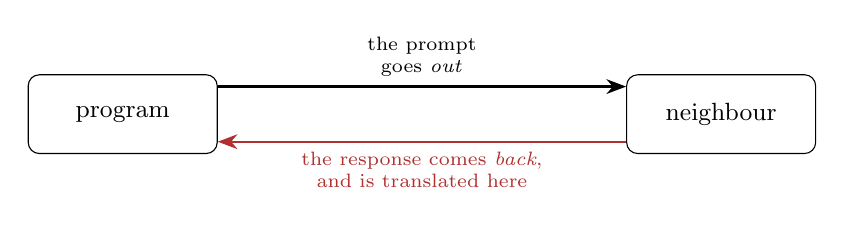
\begin{tikzpicture}[>={Stealth[length=2.5mm]}, every node/.style={font=\small}]
  \node[draw,rounded corners,minimum width=24mm,minimum height=10mm] (P) at (0,0) {program};
  \node[draw,rounded corners,minimum width=24mm,minimum height=10mm] (Q) at (7.6,0) {neighbour};
  \draw[->,thick] ([yshift=3.5mm]P.east) -- ([yshift=3.5mm]Q.west)
    node[midway,above,font=\scriptsize,align=center]{the prompt\\goes \emph{out}};
  \draw[<-,thick,bad] ([yshift=-3.5mm]P.east) -- ([yshift=-3.5mm]Q.west)
    node[midway,below,font=\scriptsize,align=center]{the response comes \emph{back},\\and is translated here};
\end{tikzpicture}
\end{center}

All three are wired this way, so the whole ring looks like this. Prompts run
one way round; every response comes back the other way, translated at each
program it passes through.

\begin{center}
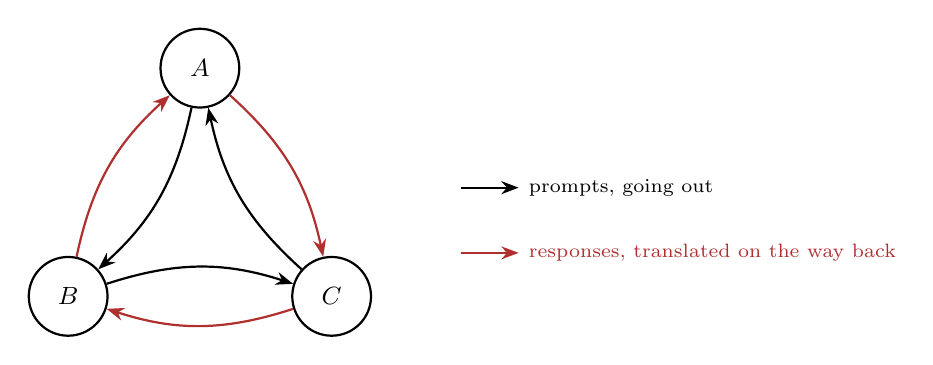
\begin{tikzpicture}[>={Stealth[length=2.2mm]}, scale=0.92,
                    every node/.style={font=\small}]
  \node[circle,draw,thick,minimum size=10mm] (A) at (90:2.1)  {$A$};
  \node[circle,draw,thick,minimum size=10mm] (B) at (210:2.1) {$B$};
  \node[circle,draw,thick,minimum size=10mm] (C) at (330:2.1) {$C$};
  \draw[->,thick] (A) to[bend left=18] (B);
  \draw[->,thick] (B) to[bend left=18] (C);
  \draw[->,thick] (C) to[bend left=18] (A);
  \draw[->,thick,bad] (B) to[bend left=18] (A);
  \draw[->,thick,bad] (C) to[bend left=18] (B);
  \draw[->,thick,bad] (A) to[bend left=18] (C);
  \draw[->,thick] (3.6,0.45) -- (4.4,0.45)
    node[right,font=\scriptsize]{prompts, going out};
  \draw[->,thick,bad] (3.6,-0.45) -- (4.4,-0.45)
    node[right,font=\scriptsize]{responses, translated on the way back};
\end{tikzpicture}
\end{center}

\section*{3. The complication: neighbours may use opposite conventions}

Each program holds a value which is either $+1$ or $-1$ --- think of it as a
measurement. The complication is that \textbf{neighbouring programs may use
opposite conventions}: two labs measuring the same quantity, one recording
depth below sea level as positive, the other as negative. Neither is wrong.
But when one passes a number to the other, somebody has to flip the sign.

So each \emph{edge} of the ring carries a label: $+$ if the two neighbours
agree about which way is up, $-$ if they are opposite. Three programs, three
edges, so the whole setup is three signs. Note \emph{where} the flip happens:
on the response, coming back. The prompt going out carries no value and needs
no translation. Hold on to that.

\begin{center}
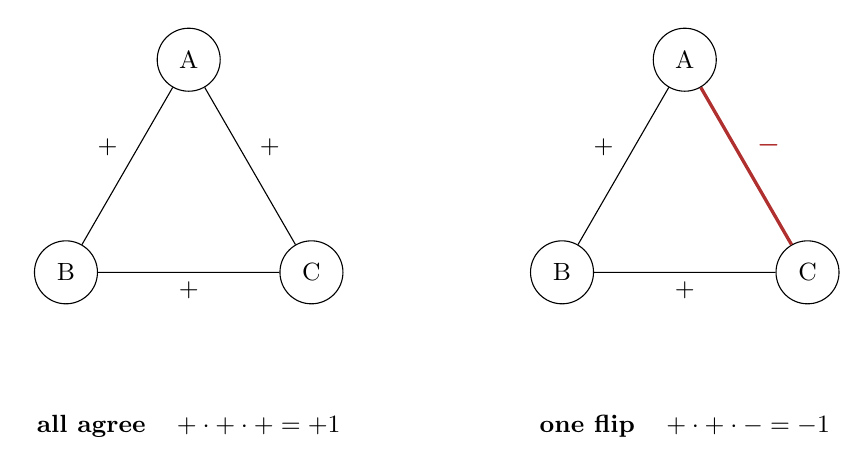
\begin{tikzpicture}[scale=1.5, every node/.style={font=\small}]
  \foreach \i/\a/\l in {0/90/A, 1/210/B, 2/330/C}
    \node[circle,draw,minimum size=8mm] (\l) at (\a:1.2) {\l};
  \draw (A) -- node[above left] {$+$} (B);
  \draw (B) -- node[below] {$+$} (C);
  \draw (C) -- node[above right] {$+$} (A);
  \node at (0,-1.9) {\textbf{all agree} \;\; $+\cdot+\cdot+ = +1$};
  \begin{scope}[xshift=4.2cm]
  \foreach \i/\a/\l in {0/90/A, 1/210/B, 2/330/C}
    \node[circle,draw,minimum size=8mm] (\l') at (\a:1.2) {\l};
  \draw (A') -- node[above left] {$+$} (B');
  \draw (B') -- node[below] {$+$} (C');
  \draw[very thick, bad] (C') -- node[above right] {$\boldsymbol{-}$} (A');
  \node at (0,-1.9) {\textbf{one flip} \;\; $+\cdot+\cdot- = -1$};
  \end{scope}
\end{tikzpicture}
\end{center}

Two interesting cases: all three edges $+$, or one edge $-$.

\subsection*{Can everybody agree on one number?}

Pick a value for $A$. Pass it from $A$ to $B$, flipping if that edge says $-$.
Pass it from $B$ to $C$ the same way. Then from $C$ back to $A$, again the same
way --- and check whether you get back what you started with.

\textbf{Multiply the three edge signs.} If the product is $+1$, you come home
with the number you left with, and the three programs can settle on one
consistent set of values. If the product is $-1$, you come home with the
opposite of what you left with, and no consistent assignment exists at all.

\begin{keybox}
\textbf{This is the time zone problem.} Each time zone is one hour ahead of its
western neighbour. Go all the way around the globe adding an hour at each step
and you arrive back where you started $24$ hours later --- a whole day out of
step with yourself. Every local agreement is correct; the global assignment is
impossible.
\end{keybox}

Two things worth noticing, because both matter later.

\textbf{Only the product matters, not which edge carries the minus.} And if one
program unilaterally flips its own convention, the two edges touching it both
change sign, so the product is unchanged. The disagreement belongs to the ring
as a whole, not to any one program's private choice. We checked this: $24$
different ways of flipping individual conventions, and the verdict never moved.

\textbf{Whether you can agree is decided entirely by a multiplication.} Three
signs, one product, two possible answers. That is the whole of the first
question.

\section*{4. Second question: does the ring ever respond?}

Now ask the ring to actually compute something. We ran two different programs
on it, and the difference between them is the whole of this section.

\subsection*{The first program: buck-passing}

Program $A$ is prompted: what is your value? Recall from \S2 that a program
responds by prompting its neighbour. So $A$ prompts $B$; $B$, responding the
same way, prompts $C$; and $C$ prompts $A$.

Call this \textbf{buck-passing}: \emph{every program in the ring responds to a
prompt only by prompting someone else, and no program anywhere has a response
of its own}. The phrase is from ``passing the buck'' --- each person handed the
prompt refuses to settle it and hands it on. In a line that is harmless,
because the last person in the line has to respond. In a ring there is no last
person.

This never finishes. It is worth being precise about how it fails, because the
obvious guess is wrong. \textbf{Nothing is stuck.} No program is waiting on a
lock, nothing has deadlocked, no prompt is blocked. Every machine is busy the
whole time. The prompt simply goes round and round, and no response ever comes
back, because no response was ever produced anywhere.

\subsection*{The second program: cutting the ring}

The obvious repair is to stop the prompts going round for ever, and the way
to do that is to stop them going round at all.

\begin{keybox}
A \textbf{cut} is one chosen edge, across which no prompt may be passed.
\end{keybox}

Choosing a cut turns the ring into a line. The two programs at the ends of that
line have only one neighbour they are allowed to prompt, and the one furthest from
where you started has nobody left to prompt at all --- so it must respond from
its own value instead of passing the prompt on. That response then travels back
along the line, translated at each step exactly as before.

\begin{center}
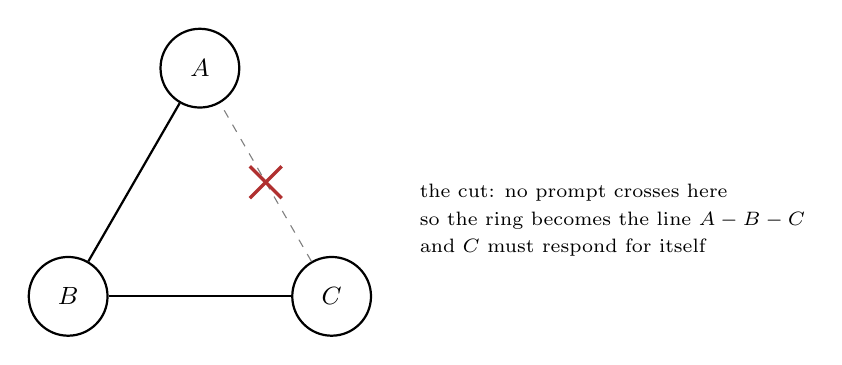
\begin{tikzpicture}[>={Stealth[length=2.2mm]}, scale=0.92,
                    every node/.style={font=\small}]
  \node[circle,draw,thick,minimum size=10mm] (A) at (90:2.1)  {$A$};
  \node[circle,draw,thick,minimum size=10mm] (B) at (210:2.1) {$B$};
  \node[circle,draw,thick,minimum size=10mm] (C) at (330:2.1) {$C$};
  \draw[thick] (A) -- (B);
  \draw[thick] (B) -- (C);
  \draw[dashed, gray] (C) -- (A);
  \node[bad, font=\large] at (330:2.1 |- 0,0.75) {};
  \draw[bad, very thick] ($(C)!0.5!(A)+(-0.22,-0.22)$) -- ($(C)!0.5!(A)+(0.22,0.22)$);
  \draw[bad, very thick] ($(C)!0.5!(A)+(-0.22,0.22)$) -- ($(C)!0.5!(A)+(0.22,-0.22)$);
  \node[align=left, font=\scriptsize, anchor=west] at (2.9,0)
    {the cut: no prompt crosses here\\[2pt]
     so the ring becomes the line $A - B - C$\\[2pt]
     and $C$ must respond for itself};
\end{tikzpicture}
\end{center}

There are three edges, so there are three possible cuts. This program always
finishes, whichever one you pick. What \S7 is about is the fact that you had to
pick.

\section*{5. The experiment}

Two questions, two configurations. Four combinations. We ran all four.

\begin{center}
\small
\setlength{\tabcolsep}{4pt}
\begin{tabular}{llccl}
\toprule
config & program & can agree? & finishes? & what happened \\
\midrule
all $+$   & buck-passing & yes & \textcolor{bad}{\textbf{no}}  & gave up after 8s, $757$ hops \\
all $+$   & cut          & yes & \textcolor{good}{yes} & all three cuts gave the same response \\
one $-$   & buck-passing & no  & \textcolor{bad}{\textbf{no}}  & gave up after 6s, $660$ hops \\
one $-$   & cut          & no  & \textcolor{good}{yes} & the three cuts gave \emph{different} responses \\
\bottomrule
\end{tabular}
\end{center}

\section*{6. The surprise}

Look at the first row.

Every edge is $+$. Everybody agrees about which way is up. A consistent
assignment exists --- there are two of them. Nothing whatsoever is obstructed.

\textbf{And the program still never finishes.} We abandoned it after eight
seconds, by which point $757$ messages had gone round the ring, and the ring was
still turning after we walked away.

So the two questions are not the same question, and this is the result:

\begin{keybox}
\textbf{Whether the programs can agree, and whether the program ever responds,
are two unrelated problems.}

You can have either one without the other. Fixing the sign disagreement does
nothing for the buck-passing, and vice versa. A working system needs both
fixed, and they need fixing by different means.
\end{keybox}

The reason is the two directions from \S1, and once you see it the whole thing is
almost disappointing.

The signs live on the \textbf{homeward direction}. They are applied to the response,
on the way back, because that is the only place a translation between two
conventions can happen.

Buck-passing lives on the \textbf{outward direction}. Whether a prompt ever
reaches somebody who will respond is decided entirely by where the prompts go
--- and the outgoing prompt carries no value, so it never touches a sign at
all.

Two failures, one in each direction. A program's two rules are chosen
independently --- which prompt you forward, and how you translate what comes
back --- and neither constrains the other. So the two failures are independent,
and that is not a quirk of this example. It is what having two rules means.

\section*{7. What the cut costs}

Cutting always terminates, in both configurations. But you had to choose which
edge to cut, and that choice is not free.

\begin{itemize}
\item \textbf{All $+$}: all three cuts give the same response. The choice was
      invisible.
\item \textbf{One $-$}: the three cuts give three different responses. The choice
      shows up in the result --- and any two of them differ by exactly the sign
      product from \S3.
\end{itemize}

\begin{keybox}
\textbf{This is the International Date Line.} You cannot have a consistent
global time without a line where the date jumps, so you draw one. It has to
exist, its position is a human decision, and the decision is visible: Samoa
moved across it in $2011$ and skipped the $30$th of December entirely.
\end{keybox}

\section*{8. The result in one sentence}

Cutting the ring buys you a response and charges you a choice, and the sign
product is exactly the size of the bill.

When the signs multiply to $+1$ the choice is free --- every cut gives the same
response, so it doesn't matter where you put the date line. When they multiply to
$-1$ the choice is real --- the response you get depends on where you cut, and
there is no cut that is more correct than the others.

The formal version checks the three claims on all eight possible sign
configurations, not a sample, plus the $24$ convention-flips.

\section*{9. Why this was worth doing}

An earlier note asked whether these two failures were secretly the same failure,
and offered two possibilities: they are the same, or one of the two ways of
describing the system is wrong.

The answer is that both descriptions are right and each is blind to half the
machine. One of them can only see whether the programs agree. The other can only
see whether the program finishes. Neither can see both, which is why asking them
to agree with each other produced no sensible answer.

\section*{Glossary}

Only if you want to read the technical version.

\begin{center}
\small
\begin{tabular}{ll}
\toprule
what this note said & what the other one says \\
\midrule
the prompts, and per prompt the response shape & a container, $S \triangleleft P$ \\
responding by prompting, and translating back & a container morphism, the pair $(u,f)$ \\
the outgoing prompt & the forward map, $u$ \\
the returning response, sign applied & the backward map, $f$ \\
can everybody agree on one number? & does a global section exist? \\
the product of the three signs & the holonomy \\
the two cases, agree / cannot agree & the class in $H^1$, trivial or not \\
flipping one program's own convention & a gauge transformation, a coboundary \\
the response doesn't depend on the cut & the section is canonical \\
the buck-passing never finishes & the composite is not well founded \\
``both descriptions see half the machine'' & the two obstructions are independent \\
\bottomrule
\end{tabular}
\end{center}

\end{document}
